\chapter{Chemotherapy}
\label{chap:chemo}

This chapter proposes a computationally guided approach to dose selection in cancer treatments.
As it is not experimentally feasible to explore the full spectrum of possible drug doses and regimens,
a mathematical framework is used to sort through the countless possible combinations.
Our approach is based upon a mathematical model that quantitatively captures the complex interactions between a tumor, the host immune system, and a chemotherapy drug.
The proposed model is calibrated with experimental data collected from \ac{SCID} mice implanted with aggressive treatment-resistant glioma tumors.  A variety of cyclopsphamide doses and schedules are considered, and data is collected on both tumor volume and immune cell markers.
After calibration, a \ac{MDOR} is computed using optimal control techniques.
For this mouse model, we find that the \ac{MDOR} that minimizes tumor size after 60 days is neither a classical metronomic schedule nor a \ac{MTD} schedule.
Instead, our \ac{MDOR} consists of administering a lower dose at the beginning of treatment, followed by a larger dose after 35 days.
The discovered regimen is analogous to the ``press-pulse'' theory in ecology.  In that theory, frequent and expansive mass species extinctions occur after ``press'' disturbances (such as climate or sea level change) weaken and destabilize populations over many generations, and are then followed by a ``pulse'' disturbance that causes extensive mortality.
This work highlights the ability of mathematical models derived from experimental data to provide insights into improved dosing and scheduling for long-term tumor reduction, to be subsequently experimentally evaluated.

\section{Introduction}
Finding the appropriate dosing and scheduling of a chemotherapy drug for a given tumor type is an exceedingly challenging task. The current standard of care limits the regimens used primarily to daily dose and \ac{MTD} treatments. A \ac{MTD} regimen attempts to reduce the tumor burden as much as tolerable by the patient with each treatment. In addition to potential severe side effects, the treatment can lose efficacy rapidly and give rise to drug resistance \cite{zahreddine2013mechanisms,kareva2015metronomic,shah2016limiting}. In addition to simply selectively killing non-resistant cells in a ``Darwin''-like fashion, high levels of cytotoxicity caused by \ac{MTD} treatments can greatly weaken the host immune system \cite{kareva2015metronomic}, removing an important line of defense against resistant cells. Metronomic or ``intermittent'' chemotherapy treatments with lower dose amount and higher frequency than \ac{MTD} were shown to be able to induce an immune response alongside the cytotoxicity of the drug towards cancerous cells, at least in mouse models, and under specific treatment conditions \cite{kepp2009immunogenic,kepp2011molecular,doloff2012vegf,kroemer2013immunogenic,vacchelli2014trial,bracci2014immune,wu2014metronomic,chen2014intermittent,bezu2015combinatorial,wu2015metronomic,wu2016metronomic}. On the other hand, if the treatments are given too regularly, such as seen in the case of daily dose treatments, the elicited immune response can be greatly attenuated \cite{wu2014metronomic}. An optimal treatment should ideally strike the right balance: eliciting a strong immune response yet still providing enough cytotoxicity towards cancer cells from the chemotherapy drug \cite{park2019goldilocks,tran2020delicate}.

Approaches like what is presented in this chapter, expanded to other mouse models and beyond, can begin to uncover optimal treatment strategies in a quantitatively-guided way,
thus addressing the stated need to explore dosing ranges earlier in the clinical trial process, as encouraged by the \ac{FDA} in Project Optimus.

\subsection{Chemotherapy drugs with immunogenic response}
Only a subset of chemotherapy drugs are known to induce an immunogenic cancer cell death pathway that produces a strong anti-cancer immune response. This effect is dependent on various factors, including the tumor type or subtype, the regimen that is being applied, and the class of chemotherapy drug. Drugs that are able to induce this type of immunostimulatory effect include cyclophopshamide, anthracyclines, 5-fluorouracil, mitoxantrone, idarubicin, and doxorubicin \cite{zitvogul2008,chen2013chemoimmunotherapy,bracci2014immune,vacchelli2014trial,pol2015trial}. In addition to using an appropriate drug, eliciting an anti-tumor immune response requires an appropriate balance of drug dosing and scheduling \cite{wu2018immunogenic,park2019goldilocks,tran2020delicate}. Much remains to be understood about the complex dynamics involved in this trade-off, as examplified by the observation of a strong immune recruitment in a 6-day repeating schedule (Q6D) at 140 mg/kg per dose of cyclophosphamide administered to treat GL261 glioma and 9L gliosarcoma tumors, a response that a daily dose or maximum tolerated treatment dose does not elicit to a noticeable extent \cite{wu2014metronomic,chen2014intermittent,doloff2012vegf}. Understanding how treatment strategies affect the dynamics and interactions between the drug, the immune system, and the tumor holds a key to developing more effective treatment strategies.

\subsection{Mathematical modeling of chemotherapy}
Developing realistic mathematical models of these biological interactions is a challenging task, since a large number of phenomena need to be considered. A detailed model of the immune system alone needs consideration of different immune cell types and chemicals (cytokines and chemokines). Even for a given cell type, the same cell may play very different roles (e.g., T-cells can be cytotoxic or memory). Each of these immune components has distinct dynamics that makes it difficult to predict the aggregate behavior of the biological system as a whole from its various components. There are additional factors to consider in therapy, such as individual variability between patients, tumor heterogeneity, the particular drug used for treatment, and how the chosen drug is administered. The fact that a cytotoxic drug like cyclophosphamide can be both immunostimulatory and immunosuppressive in a metronomic treatment makes designing accurate mathematical representations of the interactions at play particularly difficult. Although there is a rich literature on mathematical models that attempt to capture the mechanisms behind cancer chemotherapy and how it affects the immune system \cite{de2005clinical,de2006mixed,ciccolini2017pharmacokinetics,park2019goldilocks}, as well as many attempts at modeling drug resistance (see e.g.\ \cite{greene2019mathematical} and references there), the particular question that we address has been less well studied.

\subsection{Mathematically derived optimal regimen}
In this work, a computationally guided approach to dose optimization for cancer treatments is proposed that takes account of some of the introduced myriad factors. The central idea is to formulate a realistic yet simplified and phenomenological representation of the phenomena that arise during chemotherapy: drug-mediated suppression of the immune system, recruitment of immunostimulatory factors by the immunogenic cancer cell death pathway, drug resistance that arises during treatment, tumor-immune interactions, tumor growth, and drug pharmacokinetics. The parameters of the developed mathematical model are fitted to a large experimental dataset of tumor trajectories collected from \ac{SCID} mice implanted with aggressive treatment-resistant glioma tumors. A variety of cyclopsphamide doses and schedules are included in this dataset, on both tumor and immune cell markers, and treatment conditions were varied in various ranges \cite{wu2014metronomic}. 
After calibration of model parameters, we use optimal control techniques in order to compute what we call a \acf{MDOR}, derived as the strategy that minimizes tumor size at 60 days from the start of treatment. In contrast to a classical metronomic schedule or a \acf{MTD} schedule, our derived MDOR consists of administering a lower dose at the beginning of treatment, followed by a larger dose around half-way through the 60 days.

\subsection{Press-pulse theory}
An analogy can be drawn between the proposed \ac{MDOR} and the ``press-pulse'' theory in ecology, in which frequent and expansive mass species extinctions occur after ``press'' disturbances (climate or sea level change, for example) create stress so that a subsequent ``pulse'' disturbance causes extensive mortality.
Interestingly, a press-pulse therapeutic strategy for cancer management was also proposed in the very different context, that of calorie restricted ketogenic diets~\cite{2017_seyfried}, where such diets are proposed as a way to stress tumor cell energy metabolism.

\subsection{Organization of this chapter}
The rest of this paper is organized in three sections. Section~\ref{sec:methods} includes the descriptions of the mathematical model, parameter fitting, and optimal control problem setup that is used obtain the \ac{MDOR}. The mathematical model presented in this work is a modified version of the model presented in~\cite{tran2020delicate}, and, most importantly, expands the parameter fitting process to incorporate immune system data in addition to tumor volume data. The numerical optimal control results are used in the Results Section to derive a clinically feasible optimal regimen (\ac{MDOR}) and we analyze its sensitivity to dose values. The last section discusses the key findings of this paper.

\section{Methods}
\label{sec:methods}

Here a mathematical model based on the previous modeling effort~\cite{tran2020delicate} for the data set~\cite{wu2014metronomic} is introduced. The model is fitted to tumor and immune data with aa customized cost function, and used to apply optimal control techniques to find potential dosing and scheduling regimes that might be superior to the ones that were tested before. 

\subsection{Mathematical model}

The model takes into account the effects of immune recruitment, drug resistance, and the complex interactions between the drug, the tumor, and the immune system. Compared to the model introduced in \cite{tran2020delicate}, here it has been modified to become more generalizable; specific modifications and the corresponding rationale are given below.
\begin{subequations} \label{eq:chemo1}
	\begin{align} 
		\dot{T}(t) &=  k_{a} T(t) - \frac{k_{b}C(t)T(t)}{k_{c}C(t)+T(t)} - k_{d}T(t)I(t),\\
		\dot{I}(t) &= q X(t) -k_{e}T(t)I(t)-k_{f}C(t)I(t)-k_{g}Y(t)I(t)-k_{h}I,\\
		\dot{X}(t) &= \frac{q C(t)T(t)}{k_{i}C(t)+T(t)}-k_{j}X(t)-k_{k}X(t)Y(t),\\
		\dot{Y}(t) &= \frac{I(t)}{k_l+I(t)} - k_{m}Y(t) C(t),\\
		\dot{C}{t} &= u(t) - \frac{k_1 C(t)}{k_2 + C(t)}.
	\end{align}
\end{subequations}
subjected to the following initial conditions $[T,I,X,Y,C](0)=[T_0,\frac{k_n}{k_o+T_0},0,0,0]$. The unit of phenomenological variables $C$, $I$, $X$, and $Y$ is 1, and the unit of variable $T$, tumor volume, is mm$^3$. A detailed description for each parameter and variable used in this model is presented in Table~\ref{table:chemo1}.
%
\begin{landscape}
	\begin{table}
		\centering
		\caption{Definition of the variables and parameters used in the model~\eqref{eq:chemo1}.}
		\begin{tabular}{c c c c}
			\hline
			Parameter/Variable   & Unit          & Value & Definition\\ \hline
			$T(t)$       & mm$^3$         & $T(0)=T_0$& Tumor volume\\ 
			$I(t)$       & 1         & $I(0)=\frac{k_n}{k_o+T_0}$& Immune system \\ 
			$X(t)$       & 1         & $X(0)=0$ & Immunostimulatory intermediate\\ 
			$Y(t)$       & 1         & $Y(0)=0$ & Immunosuppressor intermediate\\ 
			$C(t)$       & 1         & $C(0)=0$ & Drug (input)\\ 
			$k_a$       & 1/day         & $1.555\times 10^{-1}$ & Tumor growth rate\\ 
			$k_b$       & mm$^3$/day    & $1.334\times 10^{-1}$ & Cytotoxic effect rate of the drug on the tumor\\ 
			$k_c$       & mm$^3$        & $5.195\times 10^{-1}$ & Saturation term of drug and tumor interaction \\
			$k_d$       & 1/day         & $1.992\times 10^{-2}$ & Cytotoxic effect of the immune system on the tumor \\ 
			$k_e$       & 1/day/mm$^3$  & $3.463\times 10^{-5}$ & Negative effect of the tumor on the immune system \\ 
			$k_f$       & 1/day         & $2.940\times 10^{-1}$ & Cytotoxic effect of the drug on the immune system\\ 
			$k_g$       & 1/day     & $6.497\times 10^{-1}$ & The immunosuppressor effect on the immune system\\ 
			$k_h$       & 1/day     & $1.369\times 10^{-1}$ & The immune system natural decay rate\\ 
			$k_i$       & mm$^3$    & $1.837\times 10^{-1}$ & Saturation term of the immunostimulatory recriutment term caused by the tumor debris\\ 
			$k_j$       & 1/day     & $5.987\times 10^{-4}$ & The immunostimulatory natural decay rate \\ 
			$k_k$       & 1/day     & $1.249\times 10^{-1}$ & The immunosuppression effect rate \\
			$k_l$       & 1         & $1.435\times10^{-3}$  & Saturation term of immunosuppressor increase in response to the immune system  \\ 
			$k_m$       & 1/day     & $3.997\times10^{-5}$  & Cytotoxic effect of the drug on the immunosuppressor intermediate\\
			$k_n$       & mm$^3$    & $1.966\times 10^{+3}$ & Initial immune system parameter \\ 
			$k_o$       & mm$^3$    & $2.040\times10^{-4}$  & Initial immune system parameter \\ 
			$k_1$       & 1/day     & $1.525\times 10^{+2}$ & Mechaelis-Menton elimination term parameter\\ 
			$k_2$       & 1         & $5.594\times 10^{+3}$ & Mechaelis-Menton elimination term parameter\\ 
			$q$       & 1 /day        & 1 & Makes the phenamenological variables unitless. \\ 
			\hline
		\end{tabular}
		\label{table:chemo1}
	\end{table}
\end{landscape}
%
Tumor growth inhibition data has been previously used to identify the parameters in our previous work \cite{tran2020delicate}. Here, the objective function is defined to compare the tumor and immune data for fitting the parameters in model~\eqref{eq:chemo1}. It is made up of two components: $f_1(x)$ the error with respect to the tumor data and $f_2(x)$ the error with respect to the immune data. Where $x$ is a vector of fitting parameters represented in the model and introduced in table \ref{table:chemo1}, and $X$ is the physically meaningful parameters space search defined by upper bound and lower bound of each parameter. This is to incorporate both the experimentally measured tumor growth inhibition and immune markers into the model.
%
\begin{equation} \label{objective}
	\min_{x\in X}\; \qquad w_1\times\underbrace{f_1(x)}_\textrm{based on the measured tumor volume}\;\;+\; w_2\times\underbrace{f_2(x)}_\textrm{based on the average of measured immune system markers}.
\end{equation}
%
A best set of parameters represented in table \ref{table:chemo1} are identified to result in minimum value of the objective function. To remove bias of the fitted parameters to immune or tumor data, the weights $w_1$ and $w_2$ are selected such that both error terms of similar magnitude. In this work, the values for $w_1$ and $w_2$ were picked to be 1 and 18, respectively.

For calculating the objective function the simulated tumor data and immune data are needed to be compared with the experimentally measured data. Comparing the experimental tumor data to its corresponding simulated data is obvious because they constitute similar measurements. 
In the case of the immune data, there are 18 measured correlated immune markers excluding the immunostimulatory chemokines and VEGF-A. Since there is only one variable \textit{I} accounting for the drug-induced immune response, these relative gene expression values were averaged. 

Another challenge for calculating the mean immune data in the objective function is that the experimental data was normalized as a ratio of the measured gene expression in the untreated case at a specific day. Thus, before the values are to be compared, the values of $I$ from the simulated model needs to be averaged between the different starting volumes, then normalized with respect to the simulated untreated case.

The error function used for the immune system is given by:
\begin{equation}
	f_2(x) = \frac{|I_{simulated}-I_{measured}|}{I_{measured}+\epsilon}
\end{equation}
with $\epsilon$ representing a small deviation. Where $I_{simulated}$ is the immune system level $[I(t_1), I(t_2), \dots, I(t_n)]$ at the same time points that $I_{measured}$ the immune system markers were measured $t_1, t_2, \dots, t_n$, and  $f_2(x)$ is the sum of the errors for all of the experimental immune data points.


\subsection{Immune cell markers}
A major challenge of modeling the immune system resides in the complex interactions between its components. Even using the \ac{SCID} mouse model as was used in  \cite{wu2014metronomic}, which eliminates the impact of B and T cells, maintains the impact of innate immune cells, such as NK cells, macrophages, dendritic cells, and neutrophils. An attempt to model each of these immune components individually greatly increases  model complexity and the number of parameters to be fitted, and may come even at a detriment to the model's ultimate utility. Instead, experimentally observed immune data from \cite{wu2014metronomic} can be clustered into the following three categories by response type:
\begin{enumerate}
	\item an early response from immunostimulatory chemokines (e.g. CXCL9, CXCL10, CXCL11),
	\item a correlated response from immune cell markers shortly after the release of immunostimulatory chemokines,
	\item the response of vascular endothelial growth factor A (VEGF-A), which is inversely correlated with the other measured immune cell markers.
\end{enumerate}

In Fig.~\ref{fig:immune_data}(a), we depict trends in the measured gene expression data of immune cells subject to different treatment regimens, as reported in \cite{wu2014metronomic}. As one can see in Fig.~\ref{fig:immune_data}(b), there exists a positive correlation between most immune markers with the exception CXCL9, CXCL10, CXCL11, and VEGF-A. For instance, unlike the other immune cell markers, VEGF-A (Fig.~\ref{fig:immune_data}(a)) initially decreases before increasing again, which results in negative correlation of VEGF-A and other immune cell markers. Finally, the immunostimulatory chemokines CXCL9, CXCL10 and CXCL11 are highlighted in Fig.~\ref{fig:immune_data}(c) showing how increase in their relative gene expression precedes that of immune cell markers. Using this information, we concluded that averaging the time-series data from the correlated immune markers should provide a realistic proxy for the drug-induced immune response, allowing us to proceed with a mathematical model of smaller dimensionality while preserving the key relationships observed in experimental data.

\begin{figure}
	\centering
	\begin{subfigure}[b]{\textwidth}
		\centering
		\includegraphics[width=\textwidth]{fig/chemo_wu14_immune_dataset.png}
		\caption{}
	\end{subfigure}
	\begin{subfigure}[b]{\textwidth}
		\centering
		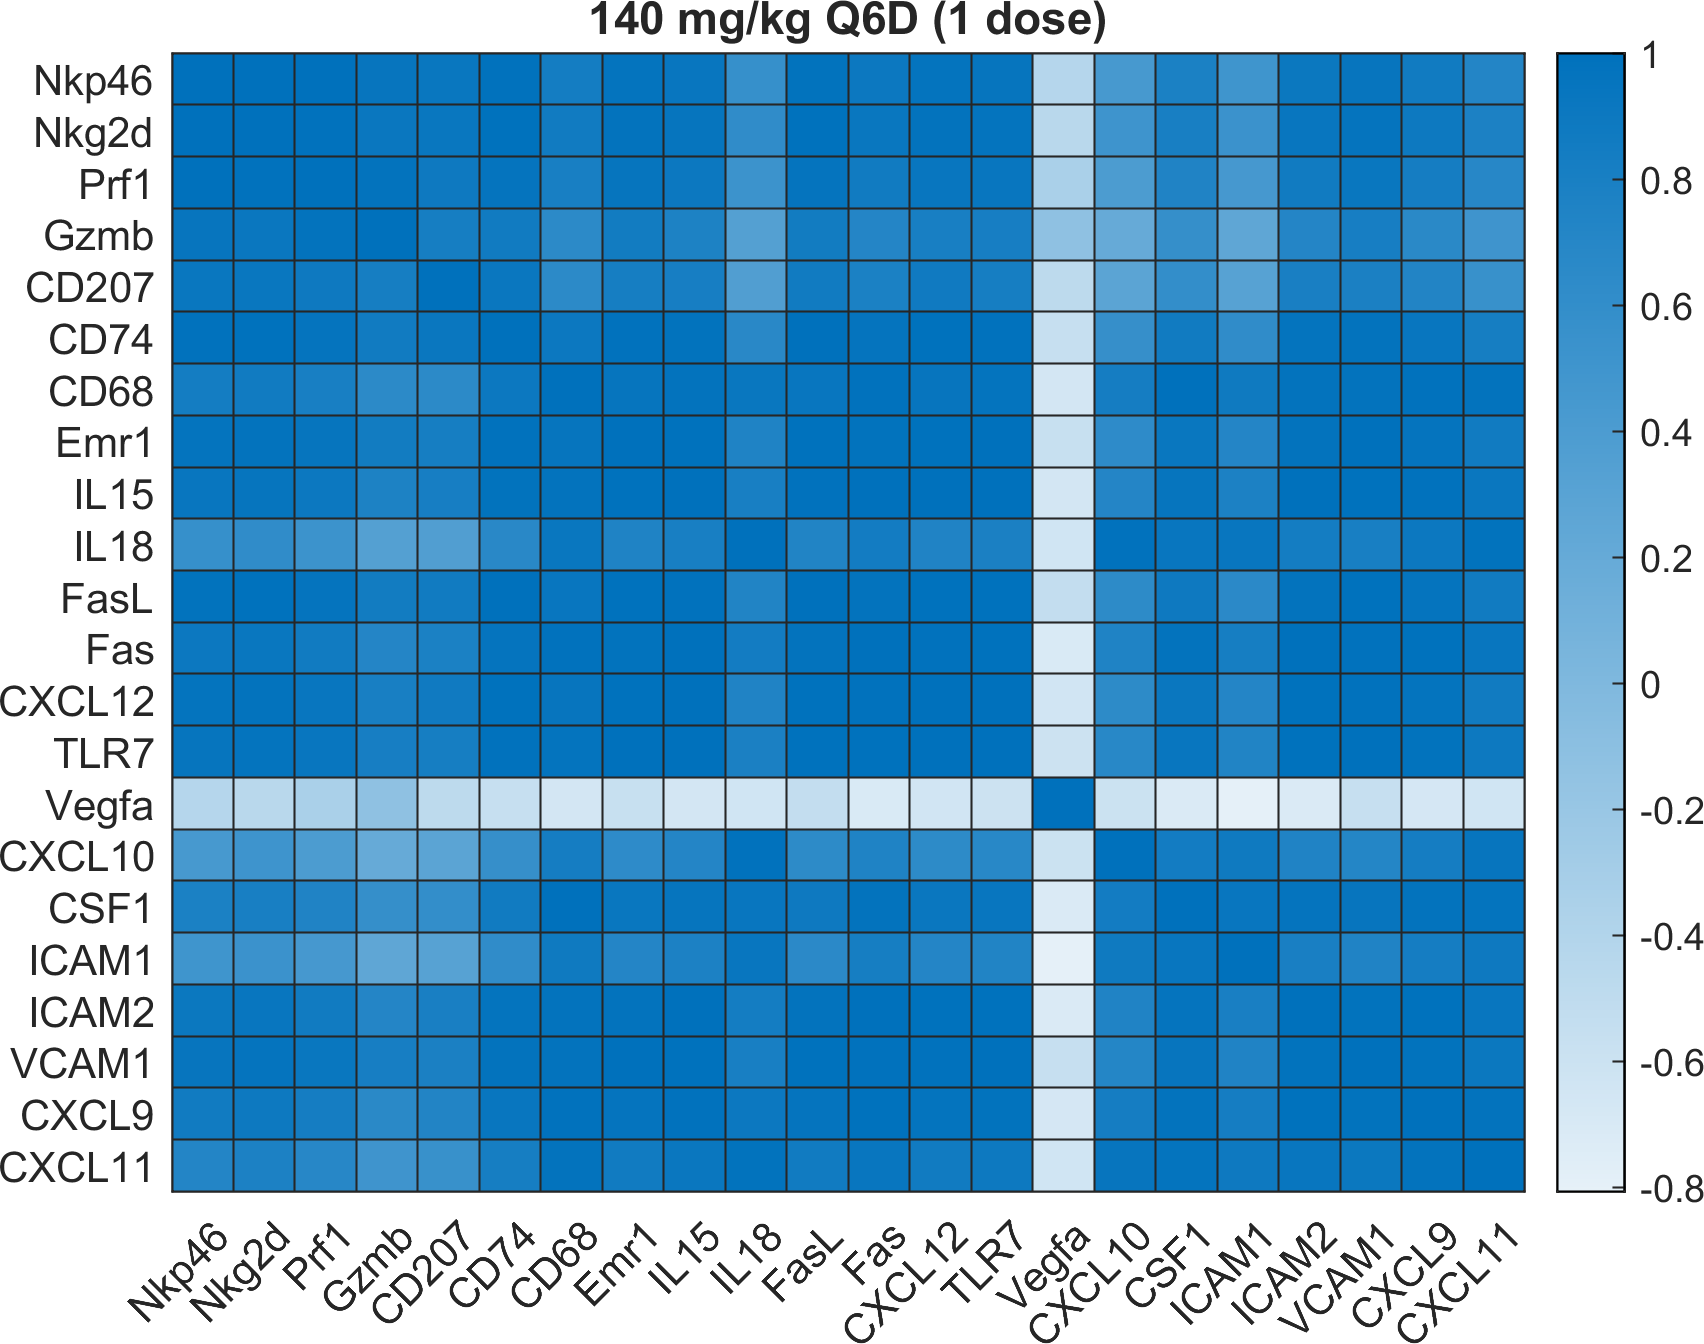
\includegraphics[width=0.3\textwidth]{fig/chemo_wu14_TD153_1CPA_corr.png}
		\includegraphics[width=0.3\textwidth]{fig/chemo_wu14_TD153_2CPA_corr.png}
		\includegraphics[width=0.3\textwidth]{fig/chemo_wu14_TD153_3CPA_corr.png}
		\caption{}
	\end{subfigure}
	\begin{subfigure}[b]{0.9\textwidth}
		\centering
		\includegraphics[width=\textwidth]{fig/chemo_wu14_immune_dataset_reordered_highlighted.png}
		\caption{}
	\end{subfigure}
	\caption[Immune cell markers]{Correlations and trends in the experimentally measured gene expression data of immune cells \cite{wu2014metronomic}. In (a), the time-series experimental data on the immune markers are shown for the 3 measured experimental conditions for which they were measured. In (b), the correlation analysis of the data in (a) is shown for the case of 1 dose and 3 doses of cyclophoshamide with a dose of 140 mg/kg and 6 days apart. In (c), the hypothesized immunostimulatory factors CXCL9, CXCL10, and CXCL11 are highlighted.}
	\label{fig:immune_data}
\end{figure}